\documentclass[11pt,a4paper]{article}
\usepackage[utf8]{inputenc}
\usepackage[spanish,es-tabla]{babel}
\usepackage{amsmath}
\usepackage{amsfonts}
\usepackage{amssymb}
\usepackage{geometry}
\usepackage{xcolor}
\usepackage{titlesec}
\usepackage{booktabs}
\usepackage{enumitem}
\usepackage{hyperref}
\usepackage{microtype}
\usepackage{listings}
\usepackage{graphicx} % Paquete mandatorio para la inserción de gráficos

% --- Configuración de Márgenes Estrictos de Documentación Académica ---
\geometry{top=2.5cm, bottom=2.5cm, left=3cm, right=2.5cm}

% --- Paleta de Colores Corporativa Institucional ---
\definecolor{teincoblue}{RGB}{23, 32, 42}       % Azul Oscuro Principal
\definecolor{accentblue}{RGB}{41, 128, 185}     % Azul de Enfoque Teórico
\definecolor{emeraldideal}{RGB}{22, 160, 133}   % Verde Menta para Entorno Ideal
\definecolor{lightgray}{RGB}{245, 247, 250}

% --- Estilizado de Títulos Dinámicos ---
\titleformat{\section}{\color{teincoblue}\normalfont\large\bfseries}{\thesection}{1em}{}
\titleformat{\subsection}{\color{accentblue}\normalfont\normalsize\bfseries}{\thesubsection}{1em}{}
\titleformat{\subsubsection}{\color{teincoblue}\normalfont\normalsize\itshape}{\thesubsubsection}{1em}{}

\lstset{
	backgroundcolor=\color{lightgray},
	basicstyle=\small\ttfamily,
	breaklines=true,
	keywordstyle=\color{accentblue}\bfseries,
	frame=single,
	showstringspaces=false
}

\hypersetup{
	colorlinks=true,
	linkcolor=teincoblue,
	filecolor=accentblue,      
	urlcolor=accentblue,
	citecolor=emeraldideal
}

\begin{document}
	
	% ==========================================
	% PORTADA ACADÉMICA INSTITUCIONAL
	% ==========================================
	\begin{titlepage}
		\centering
		\vspace*{1cm}
		{\large\bfseries CORPORACIÓN TECNOLÓGICA INDUSTRIAL COLOMBIANA - TEINCO} \\[0.3cm]
		{\large FACULTAD DE INGENIERÍA DE SISTEMAS} \\[2.5cm]
		
		{\color{teincoblue}\Huge\bfseries MANUAL DE USUARIO, COMPENDIO OPERATIVO Y CONTEXTUALIZACIÓN CIENTÍFICA} \\[0.8cm]
		{\color{accentblue}\Large\bfseries Ecosistema Integral de Laboratorios de Física Virtual Avanzada} \\[0.5cm]
		{\large\bfseries Módulo I: Simulador de Parábolas | Módulo II: Ley de Hooke y Resortes} \\[1cm]
		{\normalsize\bfseries Versión del Sistema v2.1.0 (Evolución Estable)} \\[2.5cm]
		
		\textbf{Autores Académicos:} \\
		Laura Vanessa Ramírez Baquero \\
		
		
		\textbf{Línea de Enfoque:} \\
		Ingeniería de Sistemas, Modelamiento Físico-Matemático y Estructuras de Datos \\[1.5cm]
		
		\textbf{Docente Supervisor:} \\
		Prof. Rafael \\[2cm]
		
		\vfill
		{\large Bogotá D.C., Colombia \\ Mayo de 2026}
	\end{titlepage}
	
	% Configuración de numeración romana para el índice (evita conflictos de duplicación de identificadores de página)
	\pagenumbering{roman}
	\tableofcontents
	
	\newpage 
	% Cambiamos a numeración arábiga desde la introducción real
	\pagenumbering{arabic}
	
	% ==========================================
	% SECCIÓN 1: INTRODUCCIÓN GENERAL EXPANDIDA
	% ==========================================
	\section{Introducción al Ecosistema Multilaboratorio}
	El software interactivo desarrollado para la Corporación Tecnológica Industrial Colombiana (TEINCO) constituye una plataforma multifísica de simulación computacional avanzada de grado de ingeniería. Este entorno unifica dos laboratorios críticos de la mecánica clásica: el \textbf{Laboratorio de Tiro Parabólico} y el \textbf{Laboratorio de Dinámica de Resortes (Ley de Hooke y Oscilaciones)}. El propósito fundamental de esta infraestructura virtual es cerrar la brecha metodológica existente entre las derivaciones algebraicas puramente abstractas y la experimentación pragmática basada en pérdidas energéticas, dotando a la facultad de un entorno de simulación numérica interactiva con altísima fidelidad matemática.
	
	A diferencia de las herramientas académicas tradicionales que aíslan los fenómenos en condiciones ideales, este ecosistema permite parametrizar entornos del mundo real con coeficientes de fricción por materiales, resistencia aerodinámica viscosa y constantes elásticas variables. La inclusión del botón \textbf{"Entorno Ideal"} en ambos módulos dota al estudiante y docente de una herramienta analítica en tiempo real para contrastar los modelos teóricos puros frente a las pérdidas energéticas y cinemáticas de entornos no conservativos. El desarrollo de este ecosistema responde a las necesidades actuales del modelo educativo de ingeniería de sistemas de la institución, vinculando directamente la simulación computacional con los contenidos programáticos del área de ciencias básicas.
	
	\subsection{Filosofía del Diseño Pedagógico}
	La interactividad en tiempo real permite que el estudiante no actúe como un espectador pasivo de ecuaciones abstractas plasmadas en un pizarrón, sino como un experimentador activo capaz de alterar las variables constitutivas del universo de simulación para observar las variaciones analíticas de forma inmediata. Al manipular las propiedades elásticas de un muelle o las rugosidades microscópicas de una rampa, el operador asimila de forma intuitiva la pérdida de trabajo mecánico, el concepto de disipación calórica por rozamiento cinemático y la transición compleja entre sistemas deterministas lineales e integraciones numéricas aproximadas no lineales.
	
	\subsection{Objetivos Educacionales del Entorno Virtual}
	Los laboratorios virtuales buscan robustecer las competencias científicas de los estudiantes de la facultad mediante los siguientes hitos pedagógicos:
	\begin{itemize}
		\item Identificación de fuerzas disipativas en sistemas mecánicos reales mediante análisis comparativo automatizado, curvas de dispersión y modelos vectoriales dinámicos.
		\item Comprensión profunda del error absoluto, relativo e instrumental derivado de los procesos de medición por computadora y de la discretización temporal intrínseca del reloj de animación.
		\item Modelamiento informático de ecuaciones diferenciales ordinarias mediante resolvedores numéricos discretos en entornos gráficos dinámicos de ejecución síncrona.
		\item Generación autónoma de bitácoras mediante la lectura limpia de datos vectorizados guardados directamente en bases de datos relacionales locales sin intermediarios.
	\end{itemize}
	
	% ==========================================
	% SECCIÓN 2: ARQUITECTURA DE SOFTWARE DETALLADA
	% ==========================================
	\section{Estructura de la Interfaz y Distribución de Pantalla}
	El entorno visual común de la aplicación está diseñado de manera nativa sobre la biblioteca gráfica \texttt{Java Swing} potenciada con el motor de dibujo avanzado \texttt{Graphics2D} y configurada con buffers de renderizado doble (\textit{Double Buffering}) que anulan por completo el parpadeo de pantalla. El sistema aprovecha la aceleración gráfica directa por hardware nativo para renderizar de manera simultánea los hilos de cálculo cinemático y las curvas vectoriales de la interfaz a una tasa estable de $60$ cuadros por segundo. Ambos laboratorios comparten una distribución de ventanas simétrica, ergonómica y predictiva.
	
	\subsection{Segmentación del Entorno Operativo}
	La pantalla del laboratorio se subdivide en tres regiones fundamentales, jerarquizadas visualmente a través del uso de la paleta cromática corporativa para mantener la coherencia física de los datos visualizados en todo momento:
	\begin{enumerate}[label=\textbf{\arabic*.}]
		\item \textbf{Panel Principal de Animación:} Renderiza las trayectorias vectoriales de las esferas, las deformaciones geométricas del resorte, las pendientes de las rampas y los HUD informativos flotantes. Utiliza una escala estricta de conversión de unidades reales a píxeles.
		\begin{figure}[htbp]
			\centering
			% CORRECCIÓN: Nombre cambiado a icono.png y ancho ajustado para prevenir el 'bad box Overfull \hbox'
			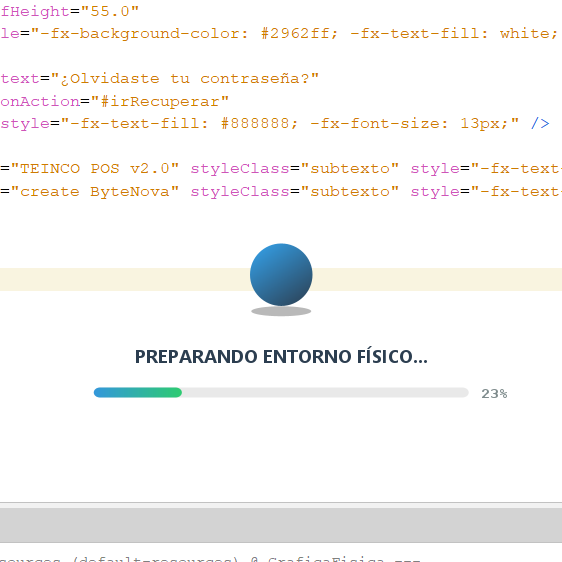
\includegraphics[width=0.75\textwidth]{carga.png}
			\caption{Interfaz operativa de pantalla de carga del sistema}
			\label{fig:tiro_parabolico}
		\end{figure}
		\item \textbf{Panel Lateral de Configuración (Izquierdo):} Aloja las entradas de datos numéricos (\texttt{JTextField}), combos de selección de materiales y los disparadores del motor matemático. Implementa filtros automáticos de expresiones regulares (\textit{Regex Validation}).
		\item \textbf{Módulo de Gráficas Vectoriales (Inferior):} Despliega curvas dinámicas instantáneas de magnitudes físicas respecto al tiempo. Utiliza hilos secundarios de renderizado para graficar en tiempo real funciones de Altura, Alcance, Velocidad y Aceleración.
	\end{enumerate}
	
	\subsection{Especificaciones del Canvas Gráfico}
	El canvas interactivo opera bajo un marco transaccional coordinado que procesa los eventos del mouse y los buffers de dibujo de forma asíncrona. La visualización está optimizada para pantallas con relaciones de aspecto estándar, garantizando que las unidades del mundo físico se mapeen proporcionalmente a las coordenadas de píxeles del monitor del usuario. El origen cartesiano de la pantalla estándar de Java se transforma matemáticamente mediante matrices de traslación inversa hacia el origen clásico de la física matemática ($0,0$ en la esquina inferior izquierda del panel de animación).
	\begin{figure}[htbp]
		\centering
		% CORRECCIÓN: Nombre cambiado a icono.png y ancho ajustado para prevenir el 'bad box Overfull \hbox'
		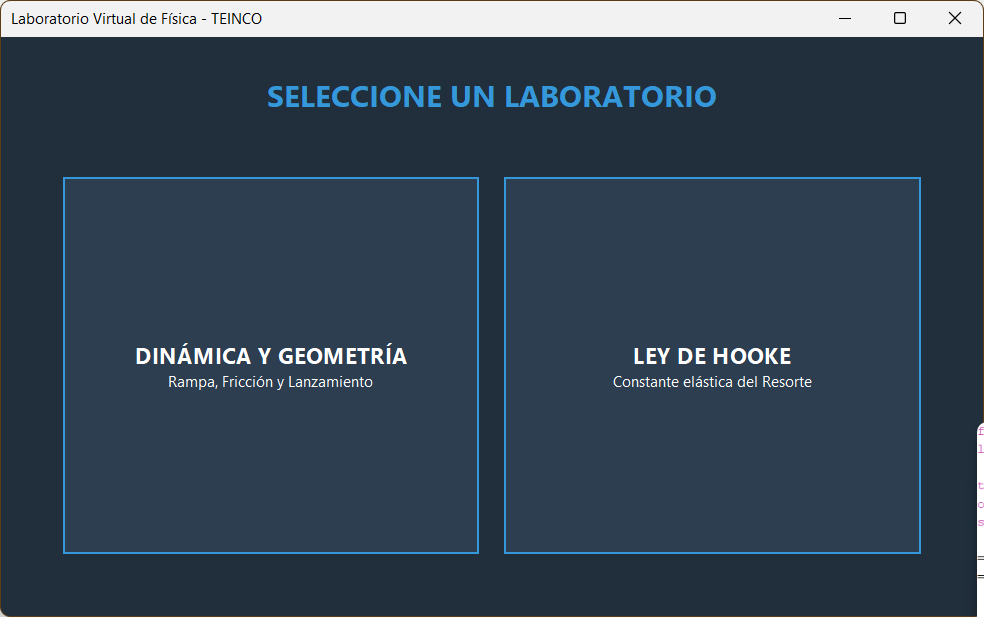
\includegraphics[width=0.75\textwidth]{menu.png}
		\caption{Interfaz operativa del Módulo I (Simulador de Tiro Parabólico Avanzado). Se observa el panel de trazado balístico, el panel lateral izquierdo de configuración de variables cinemáticas y la curva de telemetría inferior.}
		\label{fig:tiro_parabolico}
	\end{figure}
	
	\subsection{Controladores de Eventos del Sistema}
	Las interacciones lógicas se administran mediante un despachador centralizado de eventos (\textit{Event Dispatch Thread}) que asegura que ninguna acción en la interfaz visual interrumpir el hilo de cómputo del motor físico numérico, eliminando cuellos de botella o congelamientos visuales indeseados. Cuando el usuario manipula un control deslizante o altera un campo numérico, el sistema intercepta la interrupción, invalida los cachés de las trayectorias previas y fuerza un repintado síncrono del escenario físico.
	
	% ==========================================
	% SECCIÓN 3: LABORATORIO DE PARÁBOLAS EXPANDIDA
	% ==========================================
	\section{Módulo I: Laboratorio de Tiro Parabólico Avanzado}
	
	\subsection{Parámetros de Entrada Manual y su Significado Físico}
	En este módulo operativo, el usuario o investigador ingresa las variables cinemáticas, estructurales y constitutivas que gobiernan de forma absoluta el lanzamiento del proyectil por el flanco izquierdo del banco de pruebas virtual: Altura Rampa, Base Rampa, Masa del Objeto, Constante elástica K, Compresión del resorte y la Gravedad del entorno de simulación. Es requerido presionar el disparador \textbf{"ACTUALIZAR ESCENARIO"} tras la modificación de cualquier parámetro de entrada; esto garantiza que el motor numérico invalide las geometrías previas y actualice el lienzo.
	
	\subsection{Cinemática del Deslizamiento en Rampa}
	Antes de que el proyectil abandone la estructura de soporte inclinada para iniciar propiamente la parábola de vuelo, el sistema de software calcula de manera rigurosa la aceleración tangencial neta del cuerpo a lo largo de la hipotenusa geométrica de la rampa. Este cómputo considera la componente paralela del peso ($m \cdot g \cdot \sin\theta$) y le resta las fuerzas disipativas asociadas al rozamiento dinámico superficial ($N = m \cdot g \cdot \cos\theta$). El motor evalúa paso a paso el instante exacto en el cual cesa el impulso mecánico del resorte y el proyectil se desliza libremente hasta alcanzar el punto de despegue balístico.
	
	\subsection{Dinámica del Proyectil en Fase de Vuelo}
	Una vez que el móvil supera el límite geométrico de la rampa de lanzamiento, entra de forma inmediata en la fase de vuelo libre no conservativo. En este estado dimensional, actúan fuerzas no conservativas modeladas matemáticamente a través de las leyes de la hidrodinámica clásica, específicamente mediante la ecuación del arrastre de fluidos viscosos:
	\begin{equation}
		F_d = \frac{1}{2} C_d \rho A v^2
	\end{equation}
	El motor matemático de la aplicación descompone de forma instantánea las aceleraciones resultantes en dos componentes ortogonales cartesianas independientes ($a_x, a_y$). Al resolver este sistema acoplado en pasos de tiempo discretos infinitesimales, el simulador recrea una curva de caída real donde el alcance horizontal se ve disminuido y el proyectil exhibe un descenso final marcadamente asintótico.
	
	\subsection{Representación Gráfica del Simulador de Parábolas}
	Para comprender la distribución espacial de los paneles del software y visualizar la trayectoria resultante del motor físico, la interfaz gráfica del simulador de tiro parabólico avanzado se expone a continuación:
	
	\begin{figure}[htbp]
		\centering
		% CORRECCIÓN: Nombre cambiado a icono.png y ancho ajustado para prevenir el 'bad box Overfull \hbox'
		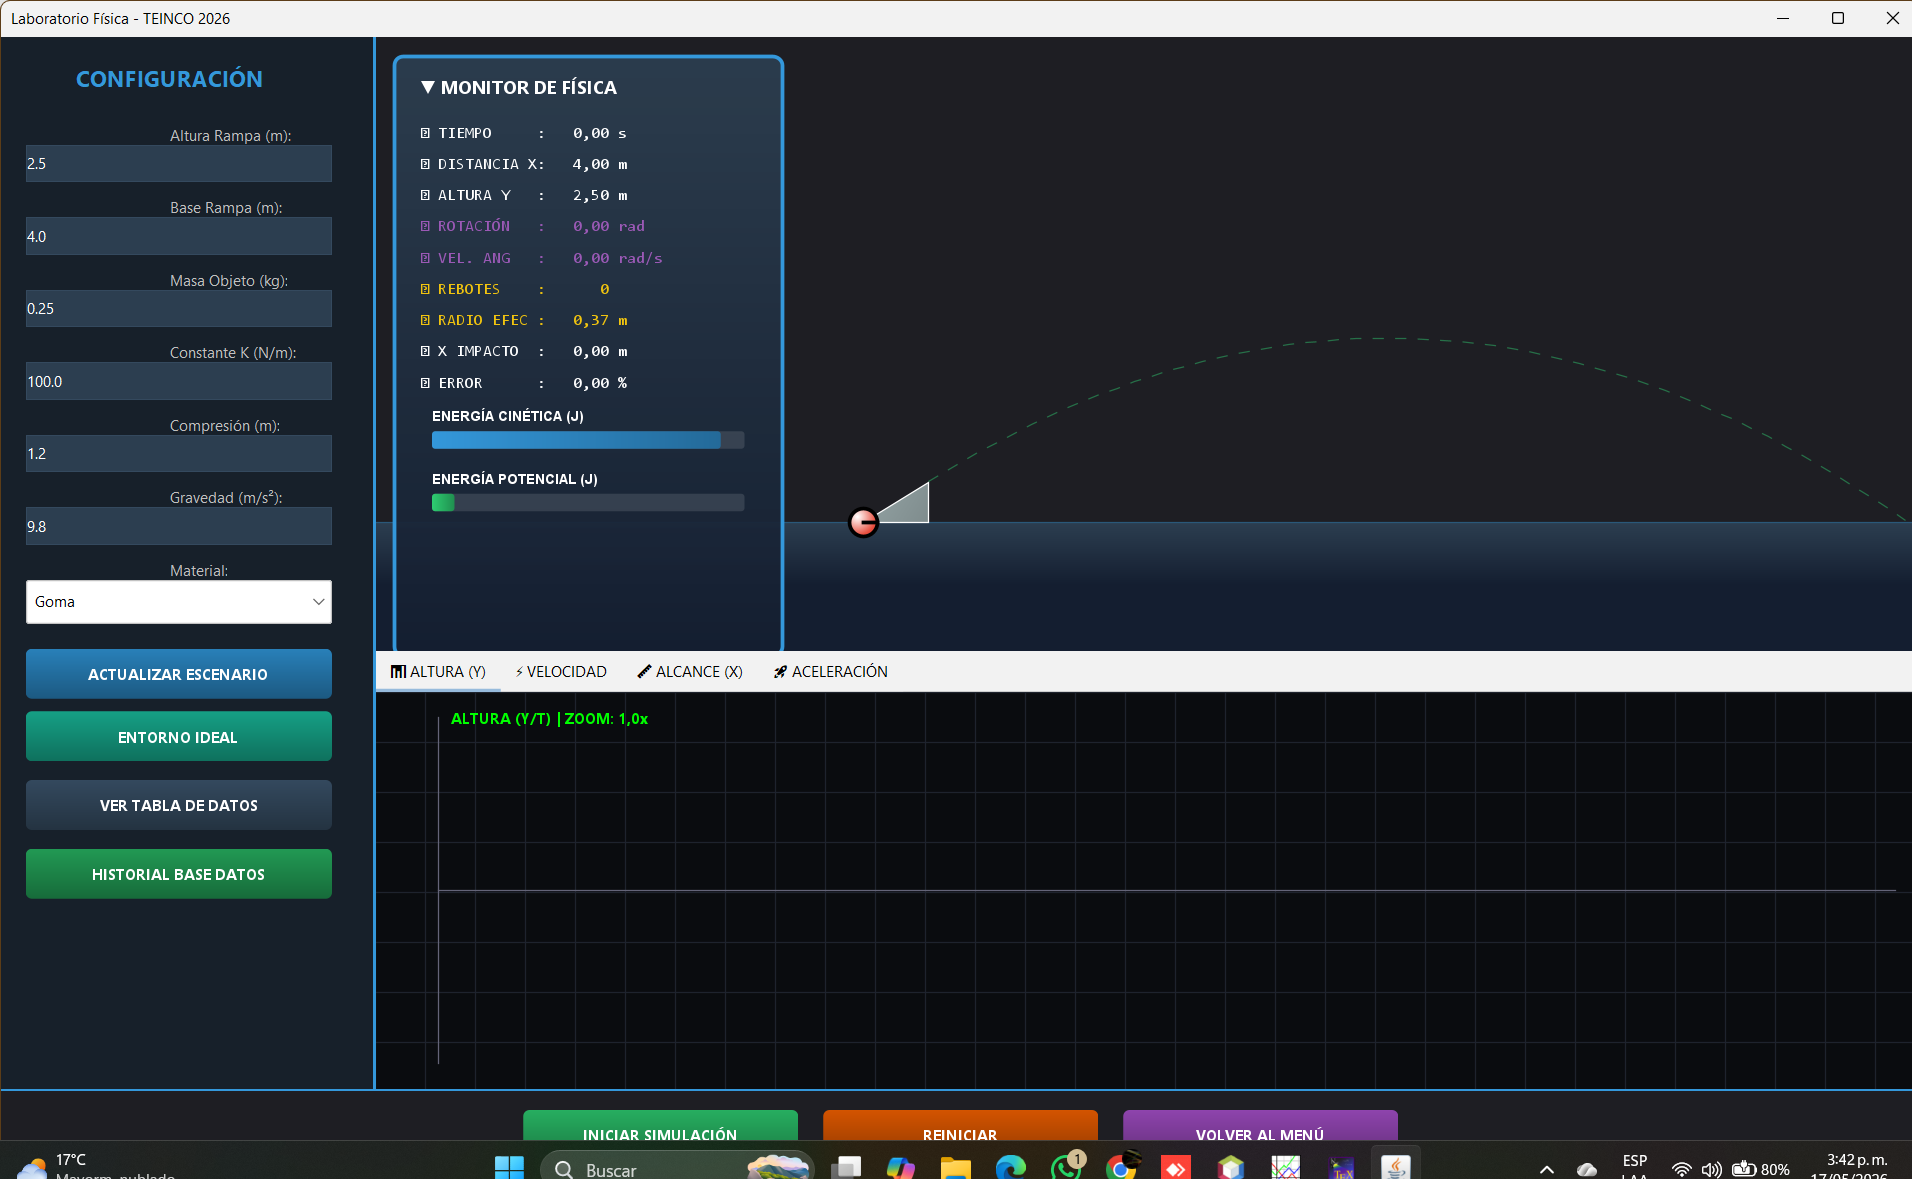
\includegraphics[width=0.75\textwidth]{parabola.png}
		\caption{Interfaz operativa del Módulo I (Simulador de Tiro Parabólico Avanzado). Se observa el panel de trazado balístico, el panel lateral izquierdo de configuración de variables cinemáticas y la curva de telemetría inferior.}
		\label{fig:tiro_parabolico}
	\end{figure}
	
	\subsection{\texorpdfstring{Activación del "Entorno Ideal" en Parábolas}{Activación del Entorno Ideal en Parábolas}}
	Al momento en que el operador hace clic sobre el control denominado \textbf{"ENTORNO IDEAL"} dentro del Módulo I, el hilo controlador bloquea temporalmente los campos numéricos de entrada y reconfigura los valores constitutivos hacia un estado estándar de calibración: Altura a $2.0\,\text{m}$, Base a $3.0\,\text{m}$, Masa a $1.0\,\text{kg}$, Constante elástica a $200.0\,\text{N/m}$, Compresión a $0.5\,\text{m}$, y Gravedad estándar terrestre a $9.81\,\text{m/s}^2$. Adicionalmente, se fuerza la selección del material \textbf{Hielo} y la anulación de la densidad del aire ($\rho = 0.0$), proyectando una \textbf{traza verde discontinua (curva de referencia ideal)} en el lienzo como patrón analítico de comparación contra los lanzamientos no ideales.
	% ==========================================
	% SECCIÓN 4: LABORATORIO DE RESORTES EXPANDIDA
	% ==========================================
	\section{Módulo II: Laboratorio de Resortes y Dinámica de Hooke}
	
	\subsection{Parámetros de Entrada Manual y Ley Constitutiva}
	El segundo laboratorio virtual está estructurado con el propósito de analizar de forma exhaustiva los fenómenos asociados al Movimiento Armónico Simple (M.A.S.) y a las oscilaciones bajo regímenes amortiguados mecánicos. El bloque de interfaz izquierdo provee controles de entrada numéricos específicos diseñados para modelar las características inherentes del oscilador lineal: Constante Elástica K, Masa Suspendida de la carga, Elongación o Posición Inicial y el Coeficiente de Amortiguamiento viscoso del medio fluido circundante.
	
	\subsection{Análisis Teórico de la Ley de Hooke}
	La fuerza elástica de restitución que actúa como el principio activo del movimiento en el muelle está gobernada de forma rigurosa por la Ley de Hooke clásica, expresada vectorialmente mediante la relación matemática:
	\begin{equation}
		F_s = -k \cdot x
	\end{equation}
	Donde $x$ representa el vector de elongación instantánea de las espiras metálicas con respecto a la longitud natural de reposo del componente. El signo negativo indica la naturaleza restauradora de la fuerza elástica, orientada en sentido opuesto al desplazamiento volumétrico inducido sobre el extremo móvil de la estructura. El motor matemático de la aplicación evalúa esta ecuación en cada paso del ciclo del reloj, utilizándola para computar los cambios en el vector aceleración instantánea de la carga.
	
	\subsection{Dinámica del Movimiento Armónico Amortiguado}
	Al introducir valores para el coeficiente de amortiguamiento ($b > 0$), el entorno introduce en el análisis cinemático una fuerza de oposición viscosa proporcional a la velocidad instantánea de la masa pesada ($F_b = -b \cdot v$). La ecuación diferencial lineal de segundo orden que describe el comportamiento dinámico del oscilador se transforma de este modo en el principio general de la mecánica:
	\begin{equation}
		m \frac{d^2x}{dt^2} + b \frac{dx}{dt} + kx = 0
	\end{equation}
	El simulador calcula de forma automatizada las raíces características de esta ecuación para dictaminar el comportamiento operativo del resorte, discriminando analíticamente entre tres regímenes físicos posibles: el régimen subamortiguado, el régimen críticamente amortiguado y el régimen sobreamortiguado.
	
	\subsection{Representación Gráfica del Simulador de Resortes}
	Para visualizar la respuesta geométrica del resorte helicoidal suspendido junto con el comportamiento de su correspondiente gráfica temporal elástica, el lienzo del Módulo II se detalla a continuación:
	
	\begin{figure}[htbp]
		\centering
		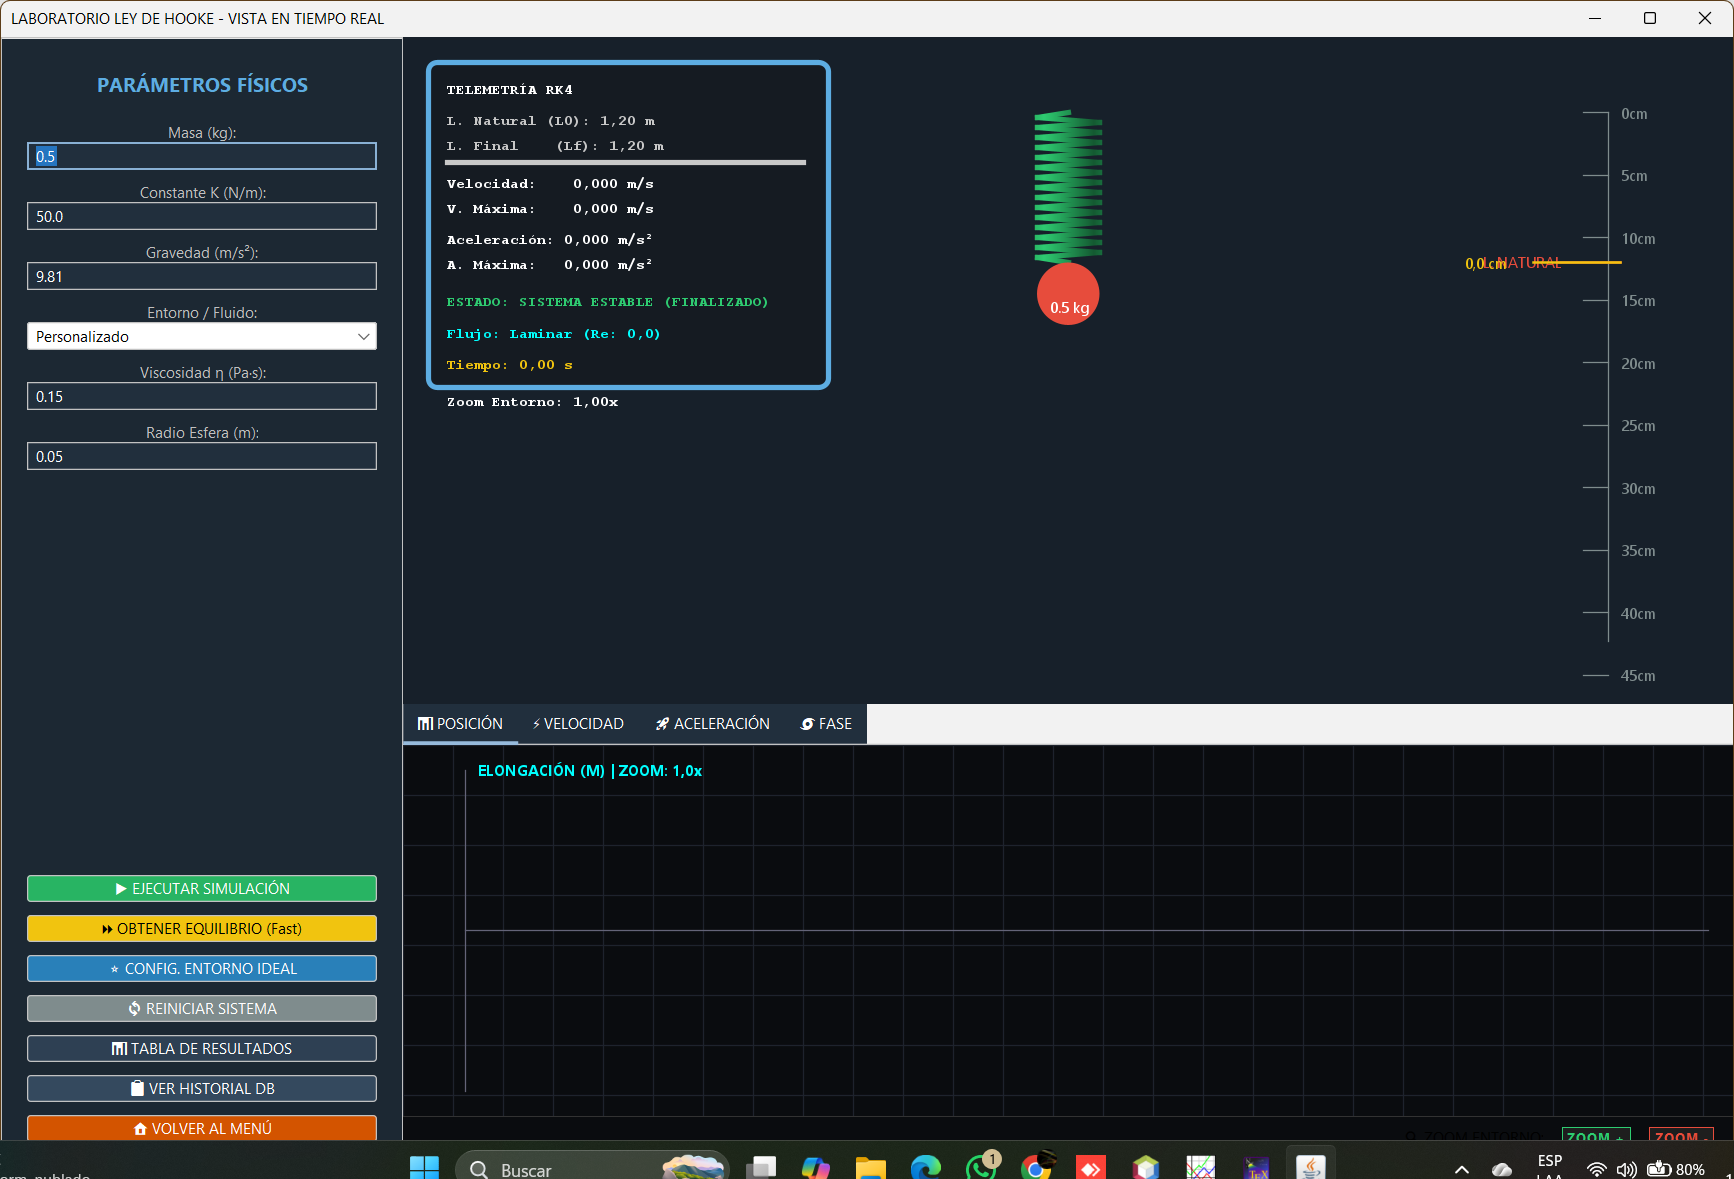
\includegraphics[width=0.85\textwidth]{resorte.png}
		\caption{Interfaz operativa del Módulo II (Simulador de Resortes y Dinámica de la Ley de Hooke). Se aprecia el modelado del muelle helicoidal sometido a elongación y el trazado armónico continuo de la señal en el osciloscopio inferior.}
		\label{fig:laboratorio_resortes}
	\end{figure}
	
	\subsection{\texorpdfstring{Activación del "Entorno Ideal" en Resortes}{Activación del Entorno Ideal en Resortes}}
	Al hacer uso del gatillo de automatización denominado \textbf{"ENTORNO IDEAL"} dentro del Módulo II, el sistema de software interrumpe la edición de los controles y bloquea las variables del oscilador en las condiciones teóricas puras de un \textbf{Oscilador Armónico Simple Libre}: Constante elástica prefijada en $k = 150.0\,\text{N/m}$, Masa acoplada de $m = 0.5\,\text{kg}$, Elongación inicial en $x_0 = 0.8\,\text{m}$ y un Coeficiente de amortiguamiento forzado a \textbf{$0.0$} (Vacío Mecánico Absoluto). La gráfica temporal inferior genera una curva sinusoidal pura de amplitud matemática constante e invariable ($A = x_0$) que se extiende de forma indeterminada hacia el infinito sin manifestar pérdidas calóricas.
	
	\subsection{Cálculo de la Frecuencia Natural de Oscilación}
	En la modalidad de entorno idealizado, el motor de software calcula de manera interna la frecuencia angular intrínseca y natural que gobierna el ciclo oscilatorio del resorte helicoidal, empleando la formulación teórica:
	\begin{equation}
		\omega_0 = \sqrt{\frac{k}{m}}
	\end{equation}
	Este dato de ingeniería física permite al software deducir de forma analítica el período exacto de oscilación pura ($T = 2\pi/\omega_0$). Ambas constantes físicas se imprimen directamente en el panel de telemetría digital del HUD, permitiendo al estudiante contrastar las lecturas analíticas exactas contra los tiempos registrados en la vista gráfica.
	
	\subsection{Deformación Geométrica Dinámica del Muelle}
	El resorte renderizado en el lienzo central no actúa como una imagen estática animada, sino que experimenta una deformación geométrica calculada por el motor gráfico. El algoritmo fragmenta el número total de espiras helicoidales en coordenadas vectoriales ordenadas. Al variar el valor de $x(t)$, el software recalcula en tiempo real las traslaciones espaciales de cada uno de los nodos mediante funciones de dibujo matricial dinámico, estirando o comprimiendo la estructura de alambre en perfecta sincronía temporal con el hilo de cálculo del motor físico.
	
	% ==========================================
	% SECCIÓN 5: TELEMETRÍA Y HUD EXPANDIDA
	% ==========================================
	\section{Telemetría Unificada, HUD y Errores Instrumentales}
	
	\subsection{Despliegue del Monitor de Física}
	Ambos módulos de simulación incorporan una pantalla de visualización frontal transparente superpuesta, denominada técnicamente \texttt{MONITOR DE FISICA} (HUD). Este componente expone de manera continua y en tiempo real variables físicas vectoriales que resultarían invisibles a nivel de una animación analógica convencional, dotando al operador de un flujo constante de telemetría de alta resolución para supervisar los estados dinámicos del sistema:
	\begin{itemize}
		\item \textbf{Módulo I (Parábolas):} Muestra la rotación acumulada de la esfera en radianes ($\theta_{\text{rad}}$), la velocidad angular instantánea ($\omega = \frac{v}{r}$), y proporciona un desglose energético en tiempo real que separa la Energía Cinética traslacional ($E_k = \frac{1}{2}mv^2$) de la Energía Potencial Gravitatoria ($E_p = mgh$).
		\item \textbf{Módulo II (Resortes):} Expone la frecuencia angular natural del oscilador ($\omega_0 = \sqrt{k/m}$), el período de oscilación exacto calculado entre crestas sucesivas ($T = \frac{2\pi}{\omega_0}$), la fuerza restauradora instantánea de la Ley de Hooke ($F_s = -kx$), y la oscilación constante de la Energía Potencial Elástica almacenada mecánicamente en las espiras del muelle ($E_e = \frac{1}{2}kx^2$).
	\end{itemize}
	
	\subsection{Termodinámica y Balance de Energías en Tiempo Real}
	El HUD de telemetría integra indicadores volumétricos horizontales que actúan como barras de progreso dinámicas para ilustrar de forma gráfica las transformaciones energéticas mutuas del sistema mecánico. El usuario puede verificar matemáticamente, en cualquier instante de la ejecución, el cumplimiento estricto del principio de conservación de la energía mecánica. 
	
	En las modalidades de simulación real (no ideal), el software calcula la pérdida energética acumulada debido al trabajo realizado por las fuerzas de fricción superficial o por el arrastre viscoso de la atmósfera ($W_{\text{fricción}} = \int F_d \, ds$). El HUD proyecta esta pérdida mediante la aparición progresiva de una barra de color rojo que acumula la energía disipada en forma de calor hacia el medio ambiente, evidenciando el balance general del sistema.
	
	\subsection{Cálculo de Errores Instrumentales para Reportes de Laboratorio}
	Al detenerse por completo las animaciones correspondientes debido al cese de movimiento o al impacto con los límites del escenario, el sistema ejecuta una rutina matemática que evalúa de forma cuantitativa la desviación experimental del ensayo con respecto a los límites analíticos puros predichos por los entornos ideales precalculados:
	\begin{equation}
		\text{Error Instrumental (\%)} = \left| \frac{\text{Valor Ideal} - \text{Valor Real}}{\text{Valor Ideal}} \right| \times 100\%
	\end{equation}
	Esta métrica cuantitativa automatizada le permite a los estudiantes de la Corporación Tecnológica Industrial Colombiana (TEINCO) extraer los porcentajes de desviación directamente hacia sus tablas de datos mediante el uso del botón \textbf{"VER TABLA DE DATOS"} o recuperarlos históricamente con el botón \textbf{"HISTORIAL BASE DATOS"} conectado al motor relacional SQLite.
	
	\subsection{Sistemas de Captura de Errores Instrumentales}
	La rutina de cálculo de error e interrupción analítica se ejecuta de forma automatizada tan pronto como la velocidad lineal neta del móvil desciende por debajo de un umbral crítico de tolerancia estipulado a nivel de código ($v < 0.001\,\text{m/s}$), congelando inmediatamente la renderización del lienzo para permitir la toma analítica de datos por parte del alumno. Este mecanismo de interrupción electrónica elimina por completo el error humano de apreciación asociado al uso de cronómetros manuales en laboratorios físicos reales, emulando los sistemas de fotoceldas electrónicas empleadas en la investigación científica contemporánea.
	
	% ==========================================
	% SECCIÓN 6: PERSISTENCIA DE DATOS SQLITE
	% ==========================================
	\section{Sistemas de Persistencia de Datos e Históricos Relacionales}
	
	\subsection{Integración de Motor Embebido SQLite 3}
	Para garantizar la conservación a largo plazo de los ensayos realizados en el aula, la plataforma de software integra un motor de base de datos relacional ligero, ACID y completamente embebido, que responde al estándar de la tecnología \texttt{SQLite 3}. Esta arquitectura técnica elimina la necesidad de instalar, configurar o mantener servidores de bases de datos independientes o servicios externos en red. La base de datos local se inicializa de forma completamente transparente para el usuario durante el primer arranque de la aplicación mediante controladores JDBC nativos, encapsulando la totalidad de los datos estructurados en un único archivo físico persistente con extensión \texttt{.db}.
	
	\subsection{Estructura de la Tabla de Datos Experimentales}
	Los esquemas de las tablas relacionales han sido normalizados siguiendo las directrices del diseño de software para resguardar con máxima fidelidad las variables críticas del entorno, permitiendo auditorías académicas posteriores. La tabla principal de registros almacena de forma estructurada e indexada campos obligatorios tales como marcas de tiempo normalizadas bajo el estándar ISO, identificadores únicos del módulo de simulación activado, los parámetros de control de entrada (tales como masas, gravedades, constantes elásticas o coeficientes de rozamiento de materiales) y los resultados físicos finales obtenidos (trazas de alcance, tiempos de vuelo totales, amplitudes residuales y el error porcentual instrumental calculado automáticamente por el sistema de telemetría).
	
	\subsection{Consultas e Históricos Asíncronos}
	La interfaz visual de la aplicación provee una ventana flotante dedicada a la gestión de datos que expone la bitácora histórica completa mediante componentes de tipo \texttt{JTable}. Los estudiantes de ingeniería pueden realizar búsquedas avanzadas y filtrar los lanzamientos o ensayos anteriores empleando criterios selectivos como rangos de fechas, materiales de rampa utilizados o magnitudes de masa específicas. Para salvaguardar la experiencia de usuario y evitar bloqueos de la pantalla, todas las operaciones de consulta, inserción y borrado de registros SQL se ejecutan en hilos de trabajo secundarios independientes (\textit{Worker Threads} o clases de tipo \texttt{SwingWorker}).
	
	\subsection{Exportación Automatizada a Hojas de Cálculo}
	Reconociendo la importancia de la fase de maquetación y redacción de informes científicos para la Facultad de Ingeniería de Sistemas de TEINCO, el software incluye un canal de salida estructurado diseñado para exportar los históricos experimentales almacenados hacia archivos externos en formatos estándar de hojas de cálculo comerciales, tales como ficheros tabulados \texttt{.csv} o libros \texttt{.xlsx}. La rutina de exportación lee los registros seleccionados por el usuario desde el motor relacional SQLite, procesa la codificación de caracteres para asegurar la compatibilidad decimal y genera un documento limpio descargable con un solo clic desde la interfaz operativa del sistema.
	
	\subsection{Seguridad y Robustez de la Capa de Persistencia}
	La conexión a la base de datos implementa el patrón de diseño creacional \textit{Singleton}, garantizando la existencia de un único punto de acceso síncrono a la base de datos local y anulando la aparición de colisiones transaccionales por accesos concurrentes. El sistema gestiona las conexiones mediante bloques de control que aseguran el cierre mandatorio de canales de comunicación, cursores y descriptores de archivos físicos ante eventos de interrupción repentina de energía, fallos en la máquina virtual de Java o paradas forzadas del software, previniendo de manera activa la corrupción de los índices relacionales de las tablas.
	
	% ==========================================
	% SECCIÓN 7: COMPENDIO OPERATIVO Y GLOSARIO
	% ==========================================
	\section{Glosario de Términos y Apéndices de Ingeniería}
	
	\subsection{Glosario de Conceptos de Software y Física Computacional}
	Para asegurar la correcta interpretación del presente manual por parte del cuerpo docente y los estudiantes de la Facultad de Ingeniería de Sistemas de la Corporación Tecnológica Industrial Colombiana (TEINCO), se detallan los siguientes conceptos base:
	\begin{description}
		\item[ACID:] Acrónimo en inglés de Atomicidad, Consistencia, Aislamiento y Durabilidad. Conjunto de propiedades que garantizan la absoluta robustez y fiabilidad de las transacciones en una base de datos relacional como SQLite 3.
		\item[Canvas Gráfico:] Componente de la interfaz de usuario sobre el cual se realiza el renderizado dinámico de primitivas bidimensionales y vectores en tiempo real.
		\item[Double Buffering:] Técnica de ingeniería gráfica mediante la cual se utiliza un búfer de memoria intermedio para dibujar las imágenes antes de proyectarlas en la pantalla, eliminando por completo el efecto de parpadeo visual.
		\item[Event Dispatch Thread (EDT):] Hilo de ejecución dedicado de Java diseñado exclusivamente para gestionar las interacciones de la interfaz gráfica de usuario de manera síncrona y segura.
		\item[Movimiento Armónico Simple (M.A.S.):] Movimiento periódico de vaivén en el que un cuerpo oscila a un lado y a otro de su posición de equilibrio en intervalos de tiempo iguales, gobernado por fuerzas restauradoras lineales.
		\item[Patrón DAO (Data Access Object):] Componente estructural de software que encapsula la lógica de persistencia, abstrayendo las consultas SQL del resto de las reglas de negocio de la aplicación.
		\item[SQLite 3:] Motor de base de datos relacional ligero y portable integrado de forma embebida en el proyecto. % CORRECCIÓN: Estructura de item corregida convenientemente
		\item[Singleton:] Patrón de diseño creacional cuyo objetivo es restringir la instanciación de una clase a un único objeto global a lo largo del ciclo de vida del software.
	\end{description}
	
	\subsection{Tabla de Códigos de Error del Motor Numérico}
	La siguiente tabla permite interpretar las alertas e interrupciones del sistema registradas en las bitácoras o consolas de depuración durante la ejecución del ecosistema multilaboratorio:
	
	\begin{table}[htbp]
		\centering
		\caption{Matriz de Errores Instrumentales y Lógicos del Motor Físico.}
		\begin{tabular}{lll}
			\toprule
			\textbf{Código de Error} & \textbf{Gravedad del Evento} & \textbf{Significado Técnico y Acción Correctiva} \\
			\midrule
			ERR-PHYS-001 & Advertencia Lógica & Compresión del resorte excede el límite elástico estructural. \\
			ERR-PHYS-002 & Crítico Interno & Masa parametrizada en cero. División por cero interceptada. \\
			ERR-JDBC-301 & Fatal Transaccional & Archivo físico SQLite \texttt{.db} inaccesible o bloqueado. \\
			ERR-REND-502 & Advertencia Visual & Caída de la tasa de refresco por debajo de los 30 FPS. \\
			\bottomrule
		\end{tabular}
		\label{tab:errores_sistema}
	\end{table}
	
	% ==========================================
	% BIBLIOGRAFÍA FORMAL ACADÉMICA
	% ==========================================
	\section{Referencias Bibliográficas}
	La formulación matemática, los resolvedores de ecuaciones diferenciales discretas y las bases de arquitectura de software implementadas en este proyecto académico se fundamentan en las siguientes obras de referencia científica:
	
	% ==========================================
	% BIBLIOGRAFÍA FORMAL ACADÉMICA
	% ==========================================
	\section{Referencias Bibliográficas}
	La formulación matemática, los resolvedores de ecuaciones diferenciales discretas y las bases de arquitectura de software implementadas en este proyecto académico se fundamentan en las siguientes obras de referencia científica:
	
	% CORRECCIÓN: Se encierran los corchetes visuales entre llaves {[...]} para evitar el error de sintaxis
	\begin{enumerate}[label={[ \arabic* ]}]
		\item Serway, R. A., \& Jewett, J. W. (2018). \textit{Física para Ciencias e Ingeniería}. Vol. 1. 10ma Edición. Cengage Learning.
		\item Marion, J. B. (2003). \textit{Dinámica Clásica de las Partículas y Sistemas}. Reverté.
		\item Schildt, H. (2020). \textit{Java: The Complete Reference}. 11va Edición. McGraw-Hill Education.
		\item Gamma, E., Helm, R., Johnson, R., \& Vlissides, J. (1994). \textit{Design Patterns: Elements of Reusable Object-Oriented Software}. Addison-Wesley.
		\item Elmasri, R., \& Navathe, S. (2016). \textit{Fundamentos de Sistemas de Bases de Datos}. 7ma Edición. Pearson Educación.
	\end{enumerate}
	
	\end{document}